\documentclass[11pt,aspectratio=169]{beamer}

% -------------------- THEME & LAYOUT --------------------
\usetheme{Madrid}
\usecolortheme{dolphin} % base color scheme
\usefonttheme{professionalfonts}
\setbeamercovered{transparent}
\setbeamertemplate{navigation symbols}{}   % remove navigation buttons
\setbeamertemplate{caption}[numbered]      % numbered captions
\setbeamertemplate{itemize items}[triangle]
\setbeamersize{text margin left=1.2cm,text margin right=1.2cm} % adjust to taste
% -------------------- GLOBAL FONT SETTINGS --------------------

% 1. Force the base beamer font to small
\setbeamerfont{normal text}{size=\small}

% 2. Force math environments to follow the "small" font size
\setbeamerfont{math text}{size=\small}
\setbeamerfont{equation}{size=\small}

% 3. Redefine \normalsize itself 
% This ensures equations and lists (which look for \normalsize) use  instead.
\let\oldnormalsize\normalsize
\renewcommand{\normalsize}{\oldnormalsize\small}

% 4. Ensure lists also stay small
\setbeamerfont{itemize/enumerate body}{size=\small}
\setbeamerfont{itemize/enumerate subbody}{size=\small}
% -------------------- FONTS & TYPOGRAPHY --------------------
\usepackage[T1]{fontenc}
\usepackage[utf8]{inputenc}
\usepackage{newpxtext,newpxmath} % Palatino-like font & math
\usepackage{microtype}

% -------------------- MATH, TABLES & GRAPHICS --------------------
\usepackage{amsmath,amssymb,amsfonts,mathtools}
\usepackage{bm,booktabs,siunitx,graphicx}
\graphicspath{{./}{./figures/}}
\renewcommand{\theequation}{11.\arabic{equation}}

% -------------------- UTILITIES --------------------
\usepackage{appendixnumberbeamer}
\usepackage{ragged2e}
\usepackage{xspace}
\usepackage{csquotes}
% -------------------- Bibliography --------------------
\usepackage[backend=biber,style=authoryear]{biblatex}
\addbibresource{sources.bib}
\usepackage{xcolor}

% -------------------- HYPERREF --------------------
\hypersetup{
  colorlinks=false,
  pdfauthor={Francesca},
  pdftitle={Chapter 1 — The Value of Currency}
}

% -------------------- COLORS & EMPHASIS --------------------
\definecolor{myblue}{RGB}{0,70,140}
\definecolor{myred}{RGB}{180,30,30}
\definecolor{mygreen}{RGB}{0,120,70}
\definecolor{gold}{RGB}{184,134,11}

\setbeamercolor{title}{fg=gold}       % title page
\setbeamercolor{frametitle}{fg=gold}  % slide titles
\setbeamercolor{structure}{fg=gold}   % bullets, sections, links
\setbeamercolor{section in head/foot}{fg=gold,bg=black!10} % gold text on light background

% -------------------- FOOTLINE --------------------
\setbeamertemplate{footline}{
  \leavevmode%
  \hbox{%
    % Section links (hidden if no current section)
    \begin{beamercolorbox}[wd=0.7\paperwidth,ht=2.5ex,dp=1.5ex,leftskip=1.4em]{section in head/foot}%
      \ifx\insertsection\empty
        % nothing
      \else
        Section: \insertsection
      \fi
    \end{beamercolorbox}%
    % Frame number right
    \begin{beamercolorbox}[wd=0.3\paperwidth,ht=2.5ex,dp=1.5ex,leftskip=3.8cm]{section in head/foot}%
      \insertframenumber/\inserttotalframenumber
    \end{beamercolorbox}%
  }%
  \vskip1pt%
}



\newcommand{\highlight}[1]{\textcolor{myblue}{#1}}
\newcommand{\warning}[1]{\textcolor{myred}{#1}}

% -------------------- SHORTCUTS --------------------
\newcommand{\E}{\mathbb{E}}
\newcommand{\R}{\mathbb{R}}
\newcommand{\dd}{\mathrm{d}}
\newcommand{\mc}[1]{\mathcal{#1}}
\newcommand{\bb}[1]{\mathbb{#1}}
\newcommand{\uc}{U_c}
\newcommand{\zg}{Z_g}

% -------------------- TIGHTER DISPLAY MATH --------------------
\makeatletter
\g@addto@macro\normalsize{%
  \setlength\abovedisplayskip{8pt}%
  \setlength\belowdisplayskip{8pt}%
  \setlength\abovedisplayshortskip{6pt}%
  \setlength\belowdisplayshortskip{6pt}%
}
\makeatother
\setbeamertemplate{frametitle}{
  \nointerlineskip
  \begin{beamercolorbox}[wd=\paperwidth,ht=3.5ex,dp=1ex,center]{frametitle}
    \centering\insertframetitle
  \end{beamercolorbox}
}

% -------------------- METADATA --------------------
\title[Part I — Currency and Money]{\textbf{Part I: Currency and Money}\\[2pt]\large Chapter 1 — The Value of Currency}
\subtitle{Currency, Money, and Price-Level Determination}
\author{Francesca}
\institute{}
\date{\today}

% -------------------- SECTION ROADMAP --------------------
\AtBeginSection[]
{
  \begin{frame}
    \tableofcontents[currentsection, hideothersubsections]
  \end{frame}
}


\begin{document}
\setcounter{equation}{0}


% ===================== TITLE SLIDE =====================
\begin{frame}[plain] % 'plain' removes header/footer for the title slide

\begin{columns}[T,totalwidth=\textwidth]

% ----- Left column: Main title, professor, chapter -----
\begin{column}{0.45\textwidth}
\vspace{2cm}

% Main title
{\usebeamercolor[fg]{title}\LARGE\textbf{Monetary Economics}\\[0.3cm]
\LARGE\textbf{and Policy}} 

\vspace{0.5cm}

% Professor name and date
{\large\textit{Pierpaolo Benigno}}\\[0.1cm]

\vspace{1cm}

% Chapter and subtitle
{\usebeamercolor[fg]{frametitle}\large Chapter 11: Shortage of "Safe Assets"}

\end{column}

% ----- Right column: Image -----
\begin{column}{0.55\textwidth}
\vspace{1cm}
\centering
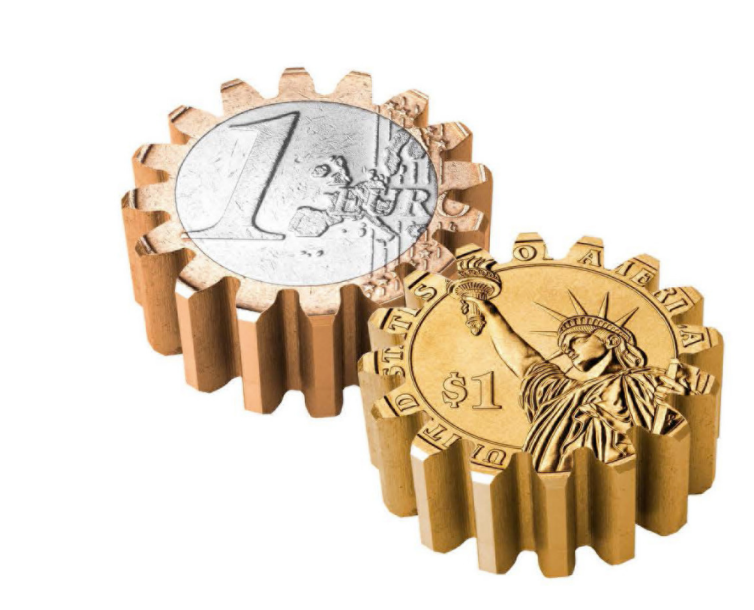
\includegraphics[width=0.9\linewidth]{Cover.png}
\end{column}

\end{columns}

% ----- Footer text (bottom-right corner) -----
\vspace*{2cm} % adjust if needed
\hfill{\large\textit{Prepared by Marcos Consuegra}}

\end{frame}

%-----------------------------------------------------------
\begin{frame}{What We Will Learn}
\small
\begin{itemize}
  \item What economists mean by \textbf{``safe assets''}: debt securities that (i) retain value in the \textbf{unit of account} and (ii) provide \textbf{liquidity services} in transactions and collateral.

  \item Why a \textbf{shortage of safe assets} shows up as a \textbf{liquidity premium} and persistently low safe interest rates.

  \item How \textbf{private intermediaries} can create \textbf{safe liabilities} in frictionless settings, and why this does \textbf{not} necessarily undermine \textbf{price-level control}.

  \item How a realistic friction, \textbf{costly monitoring} of safe investments, generates \textbf{pseudo-safe} (risky but liquid) liabilities and a \textbf{liquidity crunch} in bad states.

  \item How the \textbf{policy rate} can still stabilize prices, yet cannot by itself prevent a \textbf{collapse in real liquidity} when pseudo-safe assets default.

    \item How policy can prevent a liquidity crunch: by expanding \textbf{public liquidity} and/or backstopping private money-like claims
    through \textbf{guarantees} and regulation.

\end{itemize}
\end{frame}

% OUTLINE
\begin{frame}{Outline}
\tableofcontents
\end{frame}

%===========================================================
\section{Introduction}
%===========================================================
%-----------------------------------------------------------
\begin{frame}{Safe Assets: Definition and Liquidity Premium}
\small
\begin{itemize}
  \item \textbf{Safe assets} are financial securities that:
  \begin{itemize}
    \item retain value in terms of the currency over time,
    \item provide \textbf{liquidity services}: used for transactions and as collateral.
  \end{itemize}
  \vspace{0.45em}
  \item These services generate a \textbf{liquidity premium}:
  \begin{itemize}
    \item safe assets carry \textbf{lower interest rates} than otherwise comparable securities,
    \item the issuer finances itself on more favorable terms.
  \end{itemize}
\end{itemize}
\end{frame}

%-----------------------------------------------------------
\begin{frame}{Public vs.\ Private Production of Safe Assets}
\small
\begin{itemize}
  \item \textbf{Public production:} the central bank is the natural provider.
  \begin{itemize}
    \item In a fiat system, central bank liabilities define the unit of account and are inherently safe.
    \item Yet their supply is often \textbf{limited} relative to liquidity needs:
    \begin{itemize}
      \item domestic demand for transaction and collateral services,
      \item especially global demand when the currency is a reserve asset (e.g.\ the dollar).
    \end{itemize}
  \end{itemize}
  \vspace{0.35em}
  \item \textbf{Private production:} intermediaries can bridge the gap by issuing money-like liabilities backed by assets and equity buffers.
\end{itemize}
\end{frame}

%-----------------------------------------------------------
\begin{frame}{Another Candidate: The Sovereign}
\small
\begin{itemize}
  \item \textbf{Sovereign debt} can be a safe asset, but not for every sovereign:
  \begin{itemize}
    \item safety is an \textbf{institutional achievement}, often preceded by repeated defaults,
    \item credible repayment requires the capacity to \textbf{levy taxes} \parencite{hamilton1947,gorton2017}.
  \end{itemize}
  \vspace{0.45em}
  \item \textbf{Consolidated view} (Treasury + central bank):
  \begin{itemize}
    \item total government liabilities must be backed by taxes and/or by assets held on the public balance sheet,
    \item the riskiness of private assets held by the public sector affects the feasible tax burden.
  \end{itemize}
\end{itemize}
\end{frame}

%-----------------------------------------------------------
\begin{frame}{2007--2008: Pseudo-Safe Assets and Liquidity Collapse}
\small
\begin{itemize}
  \item \textbf{Pre-crisis:} limited supply of public safe assets encouraged private creation of money-like claims (shadow banking).
  \vspace{0.35em}
  \item \textbf{Crisis lesson:} many private claims were only \textbf{pseudo-safe}:
  \begin{itemize}
    \item liquid in good times but insufficiently backed,
    \item in the crisis they lost both value and \textbf{liquidity services}.
  \end{itemize}
  \vspace{0.35em}
  \item \textbf{Macro repercussions:}
  \begin{itemize}
    \item financial ``disequilibria'' mirror goods-market disequilibria,
    \item a \textbf{shortage of safe assets} corresponds to an \textbf{excess supply of goods}, generating falling prices and/or recession.
  \end{itemize}
\end{itemize}
\end{frame}

%-----------------------------------------------------------
\begin{frame}{A Friction in Private Safe-Asset Production}
\small
\begin{itemize}
  \item \textbf{Monitoring cost:} it is costly to identify and monitor safe investments that back private liquidity.
  \vspace{0.35em}
  \item \textbf{Financing monitoring:} intermediaries rely on the \textbf{liquidity premium}:
  \begin{itemize}
    \item the premium depends on the supply of \textbf{government liquidity},
    \item high public liquidity $\Rightarrow$ low premium $\Rightarrow$ \textbf{crowd-out} of safe private production.
  \end{itemize}
  \vspace{0.35em}
  \item \textbf{Risky debt persists:}
  \begin{itemize}
    \item risky debt is cheaper to produce (no monitoring) and can be issued abundantly,
    \item when used for liquidity, it becomes \textbf{pseudo-safe}:
    liquid in favorable states, but prone to a liquidity collapse in adverse states.
  \end{itemize}
\end{itemize}
\end{frame}

%-----------------------------------------------------------
\begin{frame}{Macroeconomic Impact of a Liquidity Crunch}
\small
\begin{itemize}
  \item When pseudo-safe assets lose backing, they default and cease to provide liquidity services:
  \begin{itemize}
    \item a \textbf{safe-asset shortage} emerges,
    \item liquidity premia and borrowing costs rise.
  \end{itemize}
  \vspace{0.35em}
  \item A collapse in money-like claims can translate into a contraction in real activity
  (in the spirit of \textcite{friedmanschwartz1963}).
  \vspace{0.35em}
  \item \textbf{Policy objective:} keep nominal spending (or broad monetary aggregates) on its pre-crisis path by offsetting the collapse in private liquidity with public intervention.
  \item Targeting nominal spending avoids having to identify every evolving form of quasi-money.
\end{itemize}
\end{frame}

%-----------------------------------------------------------
\begin{frame}{Post-2008 Policy Responses}
\small
\begin{itemize}
  \item \textbf{Public provision:} central bank asset purchases (QE) expanded reserves to satisfy demand for safe/liquid claims.
  \item \textbf{Government guarantees:} deposit insurance expansions and programs (e.g.\ FDIC guarantees) that ``harden'' private liabilities.
  \item \textbf{Regulation:} tighter capital/liquidity requirements aimed at making intermediaries' debt safer and reducing crisis likelihood.
\end{itemize}
\end{frame}


%===========================================================
\section{Outline of the results}
%===========================================================
%-----------------------------------------------------------
\begin{frame}{Outline of the Results}
\small
\begin{itemize}
  \item \textbf{Frictionless benchmarks}
  \begin{itemize}
    \item \textbf{Public supply:} with unconstrained lump-sum taxes, the government can satiate liquidity and pin down the price level.
    \item \textbf{Private supply:} with no monitoring costs ($\iota=0$), competitive intermediaries supply enough safe private debt to satiate liquidity in all states.
  \end{itemize}

  \vspace{0.35em}
  \item \textbf{Monitoring costs and pseudo-safety}
  \begin{itemize}
    \item \textbf{Shortage of private safe assets:} when monitoring is costly ($\iota>0$), safe private issuance is limited and intermediaries issue risky debt.
    \item \textbf{Pseudo-safe assets:} risky debt is liquid in good states but defaults in bad states, generating an endogenous liquidity crunch.
  \end{itemize}

  \vspace{0.35em}
  \item \textbf{Intervention and regulation}
  \begin{itemize}
    \item \textbf{Asset purchases / guarantees:} can eliminate crises and economize on taxes in good states, but crowd out truly safe private debt.
    \item \textbf{Regulation:} forcing intermediaries to hold only riskless assets removes crises but is welfare-inferior because it wastes monitoring resources.
  \end{itemize}
\end{itemize}
\end{frame}


%===========================================================
\section{Model}
%===========================================================
% --- SLIDE: Model Overview ---
%-----------------------------------------------------------
\begin{frame}{Model Overview: Structure and Risk}
\small
\begin{itemize}
  \item \textbf{Timing:} two periods, $t$ and $t+1$.
  \vspace{0.15em}
  \item \textbf{Agents:} households, financial intermediaries, and the government.
  \vspace{0.35em}
  \item \textbf{Aggregate risk at $t+1$:} two states of nature
  \[
    s\in\{h,l\},\qquad
    \Pr(h)=1-\varkappa,\qquad
    \Pr(l)=\varkappa,\qquad
    0<\varkappa<1.
  \]
  \vspace{0.2em}
  \item \textbf{Interpretation:} the low state $l$ captures a systemic event:
  risky investments fail, intermediaries default on risky liabilities, and the economy experiences a \textbf{liquidity crunch}.
\end{itemize}
\end{frame}

% --- SLIDE: Investment Technologies ---
\begin{frame}{Financial Intermediaries: Technologies}
\small
At time $t$, intermediaries choose between two distinct investment opportunities:

\vspace{0.3cm}
\begin{itemize}
  \item \textbf{Safe Technology}:
  \begin{itemize}
    \item A riskless investment that maintains its value in \textbf{both states} at $t+1$.
    \item Backs \textbf{safe private debt} which is never defaulted on.
  \end{itemize}
  \vspace{0.4cm}
  \item \textbf{Risky Technology}:
  \begin{itemize}
    \item Productive in the high state ($h$), but \textbf{loses all value} in the low state ($l$).
    \item Backs \textbf{risky private debt} which undergoes full default in state $l$.
  \end{itemize}
\end{itemize}

\end{frame}

% --- SLIDE: Assets and Payoffs ---
\begin{frame}{Households: Assets and State-Contingent Payoffs}
\small
Households can invest at time $t$ in three securities (zero-coupon, face value 1) with the following payoffs:
\begin{itemize}
  \item \textbf{Government debt $B_t$}: Always repaid (safe).
  \item \textbf{Safe private debt $S_t$}: Backed by safe projects; never defaults.
  \item \textbf{Risky private debt $D_t$}: Subject to state-contingent default:
  \begin{equation*}
    \text{payoff}(D_t) = 
    \begin{cases} 
      1 & \text{in state } h, \\ 
      0 & \text{in state } l. 
    \end{cases}
  \end{equation*}
\end{itemize}
\end{frame}

% --- SLIDE: Liquidity Services ---
\begin{frame}{Endogenous Liquidity Crisis}
\small
\textbf{Realized Liquidity Services at $t+1$}
\begin{itemize}
  \item Liquidity benefits enter the utility function via the function $V(\cdot)$.
  \item \textbf{High State ($h$)}: All assets are solvent. Realized liquidity is:
  \[ (B_t + S_t + D_t) / P_h \]
  \item \textbf{Low State ($l$)}: Risky debt defaults and ceases to provide services.
  \[(B_t + S_t) / P_l \]
\end{itemize}
\vspace{0.3cm}
\textbf{Key Assumptions on Timing}
\begin{itemize}
  \item Liquidity benefits are provided in period \textbf{$t+1$} (rather than $t$ as in Chapter 4).
  \item Therefore, this
assumption is key to modelling a liquidity crisis that occurs when the
economy switches to the low state.
\end{itemize}
\end{frame}


%------------------ Households: Preferences ------------------%
\begin{frame}{Households: Preferences}
\small
\textbf{Expected Intertemporal Utility}
\begin{equation}
C_{t}+\beta (1-\varkappa )\left[ V\left( \frac{B_{t}+S_{t}+D_{t}}{P_{h}}%
\right) +C_{h}\right] +\beta \varkappa \left[ V\left( \frac{B_{t}+S_{t}}{%
P_{l}}\right) +C_{l}\right]. \label{UtilitySafe}
\end{equation}
\vspace{0.2cm}
\textbf{Interpretation}
\begin{itemize}
    \item $C_t, C_h, C_l$: Consumption at $t$, and in states $h, l$ at $t+1$, providing linear utility.
    \item $\beta \in (0,1)$: Discount factor; $\varkappa$: Probability of the low state.
    \item $V(\cdot)$: Concave utility from real liquid services with satiation point $\bar{q} > 0$.
    \item $B_t$: Government bonds; always risk-free.
    \item $S_t$: Private Safe Assets; backed by safe technologies (no default).
    \item $D_t$: Private Risky Assets; provide liquidity in state $h$, but default in state $l$.
\end{itemize}
\end{frame}


\begin{frame}{Households: Budget Constraint at time $t$}
\small
\textbf{Budget Constraint at time $t$}
\begin{equation}
Q_{t}^{B}B_{t}+Q_{t}^{S}S_{t}+Q_{t}^{D}D_{t}+P_{t}C_{t}\leq
P_{t}Y_{t}+B_{t-1}. \label{BC0}
\end{equation}

\textbf{Interpretation}
\begin{itemize}
    \item $Q_t^B, Q_t^S, Q_t^D$: Prices of public, safe private, and risky private debt.
    \item $Y_t$: Endowment of goods at time $t$.
    \item $B_{t-1}$: Initial holdings of government bonds.
\end{itemize}

\vspace{0.3cm}
\textbf{Note}
\begin{itemize}

    \item Prices $Q_t$ represent the discount; lower prices imply higher yields.
    \item Consistent with Chapter 1, we work with prices rather than gross interest rates for tractability.
\end{itemize}
\end{frame}

\begin{frame}{Households: State-Contingent Constraints at $t+1$}
\small
\textbf{Budget Constraints at time $t+1$}
\begin{eqnarray}
P_{h}C_{h} &\leq &P_{h}Y_{h}+B_{t}+S_{t}+D_{t}+\Psi _{h}^{A}-T_{h}, \label{BCXH} \\
P_{l}C_{l} &\leq &P_{l}Y_{l}+B_{t}+S_{t}+\Psi _{l}^{A}-T_{l}. \label{BCXL}
\end{eqnarray}

\textbf{Interpretation}
\begin{itemize}
    \item $Y_{h}, Y_{l}$: State-contingent endowments at $t+1$.
    \item $T_{h}, T_{l}$: State-contingent lump-sum taxes.
    \item $\Psi_{h}^{A}, \Psi_{l}^{A}$: Aggregate profits from financial intermediaries.
\end{itemize}

\vspace{0.3cm}
\textbf{Note}
\begin{itemize}
    \item Importantly, complete default on $D_t$ is an \textbf{equilibrium outcome}, not a mere assumption.
\end{itemize}
\end{frame}

\begin{frame}{Consumption and Portfolio Choice}
\small
\textbf{Optimization Problem}
\begin{itemize}
    \item Households choose $\{C_t, C_h, C_l, B_t, S_t, D_t\}$ to maximize intertemporal utility \eqref{UtilitySafe} subject to budget constraints \eqref{BC0}, \eqref{BCXH} and \eqref{BCXL}.
\end{itemize}

\vspace{0.4cm}
\textbf{The Linear Utility Simplification}
\begin{itemize}
    \item Utility is assumed to be \textbf{linear} in consumption $C$.
    \item \textbf{Implication}: As in Chapter 4, this simplifying assumption always anchors the real interest rate to the discount factor:
    \begin{equation*}
        1+r = \frac{1}{\beta}.
    \end{equation*}
\end{itemize}
\end{frame}

\begin{frame}{Households: First-Order Conditions}
\small
\textbf{State-Contingent Liquidity Premia}
\[
\varrho_h
\equiv V_{q}\!\left( \frac{B_{t}+S_{t}+D_{t}}{P_{h}}\right),
\qquad
\varrho_l
 \equiv  V_{q}\!\left( \frac{B_{t}+S_{t}}{P_{l}}\right).
\]
\textbf{FOC for Government Bonds}:
\begin{equation}
Q_{t}^{B}=\beta \left[ (1-\varkappa )\frac{P_{t}}{P_{h}}(1+\varrho
_{h})+\varkappa \frac{P_{t}}{P_{l}}(1+\varrho _{l})\right].
\label{FOC_B}
\end{equation}
\textbf{FOCs for Private Securities}:
\begin{equation}
Q_{t}^{S}\geq \beta \left[ (1-\varkappa )\frac{P_{t}}{P_{h}}(1+\varrho
_{h})+\varkappa \frac{P_{t}}{P_{l}}(1+\varrho _{l})\right] ,
\label{FOC_S}
\end{equation}
\begin{equation}
Q_{t}^{D}\geq \beta \left[ (1-\varkappa ) \frac{P_{t}}{P_{h}}(1+\varrho _{h})%
\right] . \label{FOC_D}
\end{equation}
\end{frame}

\begin{frame}{Implications of Household FOCs}
\small
\textbf{Equilibrium Interpretation}
\begin{itemize}
    \item \eqref{FOC_B} holds with equality: since $B_t$ is in positive supply, it is always utilized for liquidity.
    \item \eqref{FOC_S} and/or \eqref{FOC_D} hold with equality when these securities are issued and used for liquidity.
\end{itemize}

\vspace{0.4em}
\textbf{Pricing Implications}
\begin{itemize}
    \item $D_t$ provides services only in state $h$ (the non-default state).
    \item Comparing \eqref{FOC_S} and \eqref{FOC_D} implies $Q_{t}^{S} \geq Q_{t}^{D}$ (safe assets command a higher price/lower yield).
    \item Liquidity services also lower the borrowing costs for issuers.
\end{itemize}
\end{frame}

\begin{frame}{Intermediaries: Technologies and Monitoring Cost}
\small
\textbf{Capital Types}:
\begin{itemize}
  \item \textbf{Safe capital $K_t^S$}: requires extra resource cost $\iota$ per unit (\textit{monitoring cost}).
  \item \textbf{Risky capital $K_t^D$}: requires no monitoring cost.
\end{itemize}

\vspace{0.2cm}
\textbf{Payoffs at $t+1$}:
\begin{itemize}
  \item \textbf{Safe capital}: produces $\frac{1}{\beta}K_t^S$ in both states $h$ and $l$.
  \item \textbf{Risky capital}: produces $\frac{A_h}{\beta}K_t^D$ in state $h$ and $0$ in state $l$.
  \item \textbf{Assumption:} Equal average productivity at $t+1$.
\end{itemize}

\vspace{0.2cm}
\textbf{Equal Average Productivity implies}:
\[
(1-\varkappa)A_h=1.
\]

\end{frame}

%------------------ Intermediaries: Market Structure ------------------%
\begin{frame}{Intermediaries: Institutional Constraints}
\small
\textbf{Market Structure and Constraints}:
\begin{itemize}
  \item Continuum of small, price-taking intermediaries.
  \item Each intermediary specializes: issues either safe debt $S_t$ or risky debt $D_t$.
\end{itemize}

\vspace{0.4cm}
\textbf{Frictions and Limited Liability}
\begin{itemize}
    \item \textbf{Limited Liability Assumption}: Intermediaries default at $t+1$ if payoffs cannot cover debt obligations.
    \item \textbf{No Equity}: Unlike Chapter 4, intermediaries cannot raise equity to buffer shocks.
\end{itemize}
\end{frame}

%------------------ Intermediaries: Safe Debt Supply ------------------%
\begin{frame}{Intermediaries: Safe Debt Supply ($S_t$)}
\small
\begin{itemize}
    \item Intermediaries issuing $S_{t}$ invest in riskless capital $K_{t}^{S}$ subject to budget constraint:
\end{itemize}

\begin{equation}
(1+\iota )P_{t}K_{t}^{S}=Q_{t}^{S}S_{t}. \label{BS1}
\end{equation}

\textbf{State-Contingent Real Profits at $t+1$}:
\begin{equation}
\Psi _{h}^{S}=\frac{K_{t}^{S}}{\beta }-\frac{S_{t}}{P_{h}} \label{PR2}
\end{equation}
\begin{equation}
\Psi _{l}^{S}=\frac{K_{t}^{S}}{\beta }-\frac{S_{t}}{P_{l}}. \label{PR1}
\end{equation}

\textbf{Supply Condition}:
\begin{itemize}
    \item Limited liability requires: $\min \left\{ \Psi _{h}^{S},\Psi _{l}^{S}\right\} \geq 0$. \label{PR3}
    \item Therefore, using \eqref{BS1} and profits \eqref{PR1}, safe debt supply is non-negative if:
\end{itemize}
\begin{equation}
Q_{t}^{S}\geq \beta \frac{P_{t}}{\min \left\{ P_{h},P_{l}\right\} }(1+\iota). \label{QSoptIntermediaries}
\end{equation}
\end{frame}

%------------------ Intermediaries: Risky Debt Supply ------------------%
\begin{frame}{Intermediaries: Risky Debt Supply ($D_t$)}
\small
\begin{itemize}
    \item Intermediaries issuing $D_{t}$ invest in risky capital $K_{t}^{D}$ subject to:
\end{itemize}

\begin{equation}
P_{t}K_{t}^{D}=Q_{t}^{D}D_{t}. \label{BS pseudo-safe}
\end{equation}

\textbf{State-Contingent Real Profits at $t+1$}:
\begin{equation}
\Psi _{h}^{D}=\frac{A_{h}}{\beta }K_{t}^{D}-\frac{D_{t}}{P_{h}}, \label{ProfitsD}
\end{equation}
\begin{equation}
\Psi _{l}^{D}=0. 
\end{equation}

\textbf{Supply Condition}:
\begin{itemize}
    \item Using \eqref{BS pseudo-safe} and the productivity assumption $(1-\varkappa )A_{h}=1$ in \eqref{ProfitsD}:
\end{itemize}
\begin{equation}
Q_{t}^{D}\geq \beta \frac{P_{t}}{P_{h}}(1-\varkappa ). \label{QD Intermediaries}
\end{equation}
\textit{\small Note: Safe capital $K^S$ could also back risky securities due to $P_h \neq P_l$ variation, but we focus on $P_h = P_l$ in equilibrium.}
\end{frame}

\begin{frame}{Entry Choice: Safe vs Risky Issuance}
\small
\begin{itemize}
  \item Intermediaries compare expected profits across the two markets.
  \vspace{0.4em}
  \item A key qualitative distinction:
  \begin{itemize}
    \item safe issuance needs a \emph{premium} to cover monitoring cost $\iota$,
    \item risky issuance can be profitable when households value liquidity in $h$.
  \end{itemize}
  \vspace{0.4em}
  \item This trade-off is the origin of pseudo-safe assets:
  \begin{itemize}
    \item liquidity provision can be abundant in good states via risky debt,
    \item but collapses in bad states due to default.
  \end{itemize}
\end{itemize}
\end{frame}

%------------------ Government ------------------%
%------------------ The Public Sector: Budget Constraints ------------------%
\begin{frame}{The Public Sector: Debt and Budget Constraints}
\small

\begin{itemize}
    \item The government balance sheet consists of liabilities ($B_t$), interpreted as Treasury debt or central bank reserves. These are inherently risk-free as they define the unit of account (see Chapter 1).
\end{itemize}
\vspace{0.2cm}
\textbf{Budget Constraint at $t$}:
\begin{equation}
Q_{t}^{B}B_{t}=B_{t-1}-T_{t}. \label{BC1}
\end{equation}

\textbf{Budget Constraint at $t+1$}:
\begin{itemize}
    \item Taxes must repay the nominal debt in both states:
\end{itemize}
\begin{equation}
T_{h}=T_{l}=B_{t}. \label{TaxesNoIntervention}
\end{equation}
\end{frame}

%------------------ Policy Rules: Monetary and Fiscal ------------------%
\begin{frame}{Policy Rules: Monetary and Fiscal Stance}
\small
\begin{itemize}
    \item We assume, as in Chapter 4, the government to follow these policies:
\end{itemize}

\vspace{0.2cm}
\textbf{Monetary Policy}
\begin{itemize}
    \item The central bank sets the interest rate on reserves at $1+i_{t}^{X}=1/\beta$.
    \item \textbf{Implication}: The bond price is anchored at $Q_{t}^{B}=\beta$.
\end{itemize}

\vspace{0.2cm}
\textbf{Fiscal Policy (Constant Real Taxes)}
\begin{itemize}
    \item The treasury maintains a constant real tax burden $b > 0$:
\begin{equation}
\frac{T_{t}}{P_{t}}=(1-\beta )b, \label{TaxS}
\end{equation}
\begin{equation}
\frac{T_{h}}{P_{h}}=\frac{T_{l}}{P_{l}}=b, \label{TaxL}
\end{equation}
for some $b>0$.
\end{itemize}

\end{frame}

%------------------ Price Level Determination ------------------%
\begin{frame}{Price Level Determination}
\small
The interaction of fiscal and monetary policies determines the path of prices.

\vspace{0.2cm}
\textbf{Constant Price Level at $t+1$}
\begin{itemize}
    \item Combining \eqref{TaxesNoIntervention} and \eqref{TaxL}, the price level is equal across contingencies:
    \[ P_{h}=P_{l}=P^{\ast}, \quad \text{where} \quad P^{\ast} = \frac{B_{t}}{b}. \]
\end{itemize}

\vspace{0.2cm}
\textbf{Determining the Price Level at $t$}
\begin{itemize}
    \item Substituting the tax policy \eqref{TaxS} into the budget constraint \eqref{BC1} yields:
\end{itemize}
\begin{equation}
\frac{B_{t-1}-\beta B_{t}}{P_{t}}=(1-\beta )b. \label{PDet9}
\end{equation}

\vspace{0.2cm}
\textbf{Note on Uniqueness}
\begin{itemize}
    \item \eqref{PDet9} provides one restriction on two unknowns ($B_t$ and $P_t$). Uniqueness requires an additional restriction coming from equilibrium in the liquidity market (through $\varrho_h,\varrho_l$ and asset demands).
\end{itemize}
\end{frame}

%===========================================================
\section{Equilibrium with the Government Satiating Liquidity}
%===========================================================

\begin{frame}{Public Satiation of Liquidity}
\small
We first analyze a baseline where the government supply of liquidity is ample enough to satisfy all domestic liquidity needs, rendering private supply irrelevant.

\vspace{0.2cm}
\textbf{The Satiation Condition}
\begin{itemize}
    \item Satiation occurs if the real tax policy $b$ is sufficiently high ($b \geq \bar{q}$).
    \item \textbf{Implication}: The marginal utility of liquidity is zero in all states:
    \[ V_{q}(\cdot )=0 \implies \varrho _{h}=\varrho _{l}=0. \]
\end{itemize}

\vspace{0.2cm}
\textbf{Asset Pricing and Price Stability}
\begin{itemize}
    \item With $\varrho=0$ and the interest-rate policy $Q_{t}^{B}=\beta$, the FOC \eqref{FOC_B} simplifies to:
    \begin{equation*}
    \beta = \beta \left[ (1-\varkappa)\frac{P_t}{P^*} + \varkappa\frac{P_t}{P^*} \right] \implies P_t = P^*.
    \end{equation*}
    \item The price level is perfectly stable over time under full government satiation.
\end{itemize}
\end{frame}

\begin{frame}{Stationary Equilibrium and "Crowding Out"}
\small
\textbf{Equilibrium Debt and Price Level}
\begin{itemize}
    \item Using $P_{t} = P^{\ast} = B_{t}/b$ in the budget restriction \eqref{PDet9}:
    \[ \frac{B_{t-1} - \beta B_t}{B_t/b} = (1-\beta)b \implies B_t = B_{t-1}. \]
    \item Consequently, the price level is determined by the initial debt stock: $P^{\ast} = B_{t-1}/b$.
\end{itemize}

\vspace{0.3cm}
\textbf{Crowding Out of Private Safe Assets}
\begin{itemize}
    \item If $\iota > 0$, intermediaries will \textbf{not} produce safe assets $S_t$.
    \item \textbf{Logic}: At satiation, there is no liquidity premium ($\varrho = 0$). Intermediaries cannot sell $S_t$ at a price high enough to cover the monitoring cost $\iota$.
    \item \textit{Result}: Only government liquidity and potentially defaulted private securities exist.
\end{itemize}
\end{frame}

%-----------------------------------------------------------
\begin{frame}{Discussion: Public Liquidity and Fiscal Limits}
\small

\textbf{Interpretation}
\begin{itemize}
  \item In this benchmark equilibrium, the government supplies enough \textbf{public liquidity} to fully satiate the economy’s liquidity needs, so that liquidity premia vanish.
  \item Private creation of safe liquidity becomes \textbf{irrelevant} (and, with monitoring costs, is crowded out).
\end{itemize}

\vspace{0.4cm}
\textbf{Critical Assumptions}
\begin{itemize}
  \item The feasibility of full liquidity satiation rests on two key requirements:
  \begin{enumerate}
    \item \textbf{Benevolence}: the government acts to maximize household welfare.
    \item \textbf{Fiscal capacity}: there are no effective limits on raising (state-contingent) taxes to back public liabilities.
  \end{enumerate}
\end{itemize}

\end{frame}

\begin{frame}{Preview: Relaxing the "No Tax Limit" Assumption}
\small
If fiscal capacity is limited ($b < \bar{q}$), a shortage arises. However, other interventions can mitigate the resulting liquidity crises:

\vspace{0.2cm}
\begin{itemize}
    \item \textbf{Alternative Tools with $b < \bar{q}$}:
    \begin{itemize}
        \item \textbf{Asset Purchases}: Central bank holds risky assets in its portfolio.
        \item \textbf{Guarantees}: Deposit insurance or public backstops.
        \item \textbf{Regulation}: Direct oversight of intermediary portfolio choices.
    \end{itemize}
    \vspace{0.4em}
    \item \textbf{Key Idea}: Risky assets provide income in good states (allowing lower taxes), but default in bad states—requiring fiscal backing exactly when crises occur.
\end{itemize}

\vspace{0.3cm}
\begin{center}
    \textit{Next: We restrict public supply ($b < \bar{q}$) to study the private creation of liquidity.}
\end{center}
\end{frame}


%===========================================================
\section{Equilibrium with No Frictions in the Supply of Private Safe Assets}
%===========================================================

\begin{frame}{Frictionless Private Supply ($\iota = 0$)}
\small
In this framework, we assume no monitoring costs for investing in risk-free projects ($\iota = 0$). 

\vspace{0.2cm}
\begin{itemize}
    \item Free entry and competition reduce all intermediary profits to zero.
    \item This implies the supply of safe \eqref{QSoptIntermediaries} and risky debt \eqref{QD Intermediaries} is non-negative at prices:
\end{itemize}
\begin{equation}
Q_{t}^{S}=\beta \frac{P_{t}}{P^{\ast }}, \qquad Q_{t}^{D}=\beta \frac{P_{t}}{P^{\ast }}(1-\varkappa ). \label{QsQD}
\end{equation}
\begin{itemize}
    \item These equations hold with equality in equilibrium due to free competition.
\end{itemize}
\end{frame}

\begin{frame}{Why an Equilibrium with Only Risky Debt Cannot Exist}
\small
\textbf{Why must private safe debt be supplied?} 
\begin{itemize}
    \item Suppose (by contradiction) intermediaries issue only risky debt $D$.
  \item In the bad state, risky debt defaults $\Rightarrow$ liquidity equals public liquidity: $\varrho_l=V_q(b)>0$.
  \item Households would attach a high value to safety, willing to pay:
  \[
    Q_t^S=\beta\left(1+\varkappa\varrho_l\right)\frac{P_t}{P^\ast} > \beta\frac{P_t}{P^\ast}.
  \]
  \item With $\iota=0$, the cost of supplying $S_t$ is only $\beta P_t/P^*$. Thus, safe issuance would yield strictly positive profits, i.e. $\varkappa\varrho_l\frac{P_t}{P^\ast}>0$.
\end{itemize}
\vspace{0.2cm}
\textbf{Contradiction}: Competition drives entry until safe debt is supplied up to the point where the premium $\varrho_l$ is eliminated.
\end{frame}

\begin{frame}{Liquidity Satiation and the First Best}
\small
Because the private sector can supply "safe assets", the economy always achieves the first best ($\bar{q}$), regardless of government fiscal capacity.

\vspace{0.2cm}
\textbf{The Resulting Liquidity Premia}
\begin{itemize}
    \item Combining supply \eqref{QsQD} with household demand \eqref{FOC_S}, we obtain:
    \begin{equation*}
    \varrho _{h}=\varrho _{l}=V_{q}\left( \frac{B_{t}+S_{t}}{P^{\ast }}\right) =0.
    \end{equation*}
    \item Even if public liquidity is scarce ($b<\bar q$), safe private debt $S_t$ expands to fill the gap.
    \item \textbf{No Liquidity Crunch}: Total safe assets remain constant across states $h$ and $l$.
\end{itemize}
\end{frame}

\begin{frame}{Price Level and Frictionless Equivalence}
\small
\textbf{Price Level Determination}
\begin{itemize}
    \item Given $Q_t^B = \beta$ and $Q_t^S = \beta P_t / P^*$, in equilibrium $P_t = P^*$.
    \item From the anchor of the price level \eqref{PDet9}, $B_t = B_{t-1}$ and the price level is determined by: $P^* = B_{t-1}/b$.
\end{itemize}

\vspace{0.4cm}
\textbf{Summary: Equivalence Result}
\begin{itemize}
    \item Frictionless private money creation does \textbf{not} impair price-level control.
    \item Private liquidity replicates the allocation achieved by full government provision.
    \item The composition of the "Safe Asset" pool is irrelevant for welfare.
\end{itemize}

\vspace{0.3cm}
% left-aligned transition line (instead of center)
\vspace{0.25cm}
{\small\textit{Next: We introduce monitoring costs ($\iota>0$), where private safe production becomes costly and ``pseudo-safe'' assets emerge.}}

\end{frame}
%===========================================================
\section{Equilibrium with Frictions in the Supply of Private Safe Assets}
%===========================================================

\begin{frame}{Monitoring Costs and the Safe Asset Shortage}
\small
We now analyze the case where intermediaries face a positive monitoring cost $\iota > 0$ when investing in risk-free projects.

\vspace{0.3cm}
\textbf{Possible Market Scenarios}
\begin{itemize}
    \item Three scenarios are theoretically possible:
    \begin{enumerate}
        \item \textbf{Safe-only}: All intermediaries issue safe debt ($S_t$).
        \item \textbf{Risky-only}: All intermediaries issue risky debt ($D_t$).
        \item \textbf{Mixed}: Both types of securities co-exist.
    \end{enumerate}
    \item We begin by proving, by contradiction, why a "safe-only" scenario cannot be an equilibrium.
\end{itemize}
\end{frame}
% --- SLIDE 1: The Break-Even Requirement ---
\begin{frame}{Infeasibility of a ``Safe-only'' Equilibrium (I)}
\small
Suppose, by contradiction, that all intermediaries issue only safe debt ($S$).

\vspace{0.3cm}
\begin{itemize}
    \item To break even, safe debt must command a liquidity premium to cover $\iota > 0$. 
    \item Equating demand \eqref{FOC_S} and supply \eqref{QSoptIntermediaries} implies:
    \begin{equation}
    \varrho_h = \varrho_l = \iota > 0.
    \end{equation}
    \item \textbf{Logic}: If $\varrho = 0$, intermediaries would make negative profits because the market price would not compensate for the monitoring cost $\iota$.
\end{itemize}
\end{frame}

% --- SLIDE 2: Symmetry and Under-provision ---
\begin{frame}{Infeasibility of a ``Safe-only'' Equilibrium (II)}
\small
\textbf{Liquidity Below Satiation}
\begin{itemize}
    \item A positive premium ($\varrho > 0$) indicates that liquidity is below the first-best level: $q < \bar{q}$.
\end{itemize}

\vspace{0.3cm}
\textbf{Symmetry Across States}
\begin{itemize}
    \item Since only safe securities (which provide equal services in both states) are issued, real liquidity is equalized:
    \begin{equation}
    q_h = q_l < \bar{q}.
    \end{equation}
    \item Consequently, state $h$ remains underserved, resulting in a positive liquidity premium: $\varrho_h > 0$.
\end{itemize}
\end{frame}

% --- SLIDE 3: The Profitable Deviation ---
\begin{frame}{Infeasibility of a ``Safe-only'' Equilibrium (III)}
\small
\textbf{Entry of Risky Debt}
\begin{itemize}
    \item Because $\varrho_h > 0$, a deviating intermediary can issue \textbf{risky debt} ($D_t$):
    \begin{itemize}
        \item It requires \textbf{no monitoring costs} ($\iota = 0$).
        \item It satisfies the liquidity demand in state $h$.
    \end{itemize}
\end{itemize}

\vspace{0.3cm}
\textbf{The Contradiction}
\begin{itemize}
    \item The intermediary earns strictly positive profits in the high state:
    \begin{equation}
    \Psi_h^D = \varrho_h \frac{D_t}{P^*} > 0.
    \end{equation}
    \item \textbf{Conclusion}: The "safe-only" scenario is not an equilibrium. Risky debt will always be supplied to capture these rents, i.e. $D > 0$.
\end{itemize}
\end{frame}

% --- SLIDE: Equilibrium in the High State ---
\begin{frame}{Equilibrium Satiation in State $h$}
\small
The "profitable deviation" logic extends to any scenario where $\varrho_h > 0$. Intermediaries will continue to supply risky debt until all potential rents are exhausted.

\vspace{0.3cm}
\textbf{The Satiation Result}
\begin{itemize}
    \item Competition in the supply of risky debt ensures that the liquidity premium in the good state vanishes:
    \begin{equation}
    \varrho_h = 0.
    \end{equation}
    \item \textbf{Efficiency}: Liquidity is at the first-best level in state $h$:
    \begin{equation}
    q_h = \bar{q}.
    \end{equation}
\end{itemize}
\end{frame}% --- SLIDE: Viability of Private Safe Assets ---
\begin{frame}{The Supply of Private Safe Assets}
\small
We have established that risky debt will be supplied. Will private safe debt be
supplied as well? 

\vspace{0.3cm}
\textbf{The Profitability Condition}
\begin{itemize}
    \item The answer is affirmative only if intermediaries can issue them at a premium to offset the monitoring cost.
    \item This depends in turn on the amount of \textbf{public liquidity}:
    \begin{itemize}
        \item \textbf{Large public supply}: Low liquidity premium on safe debt $\Rightarrow$ issuing safe debt is not profitable.
        \item \textbf{Low public supply}: Creates a profitable opportunity for intermediaries to issue safe debt.
    \end{itemize}
\end{itemize}
\end{frame}

% --- SLIDE: The Crowding-Out Condition (I) ---
\begin{frame}{The Crowding-Out Condition (I)}
\small
Intermediaries will only supply safe debt if the price investors are willing to pay covers the monitoring cost.

\vspace{0.2cm}
\textbf{Supply and Demand Prices}
\begin{itemize}
    \item To cover investment and monitoring costs, supply \eqref{FOC_B} requires:
    \begin{equation}
    Q_{t}^{S}=\beta \left( 1+\iota \right) \frac{P_{t}}{P^{\ast }}.
    \end{equation}
    \item However, from \eqref{FOC_S}, investors will \textbf{not} hold safe private debt if the price is higher than:
    \begin{equation}
    \tilde{Q}_{t}^{S}=\beta \left( 1+\varkappa \varrho _{l}\right) \frac{P_{t}}{P^{\ast }}.
    \end{equation}
\end{itemize}

\vspace{0.2cm}
\begin{itemize}
    \item Therefore, a low liquidity premium in state $l$ makes it harder to supply safe securities.
\end{itemize}
\end{frame}

% --- SLIDE: The Crowding-Out Condition (II) ---
\begin{frame}{The Crowding-Out Condition (II)}
\small

\vspace{0.4cm}
\textbf{The Crowding-Out Result}
\begin{itemize}
    \item Safe private debt will \textbf{not} be supplied if the required supply price exceeds the investor's limit ($Q_{t}^{S} > \tilde{Q}_{t}^{S}$).
    \item This occurs when the public liquidity ($b$) is high enough that:
    \begin{equation}
    V_{q}(b) < \frac{\iota}{\varkappa}.
    \end{equation}
    \item \textbf{Conclusion}: Sufficiently high public debt reduces the liquidity premium to a point where private production of safety is no longer profitable.
\end{itemize}
\end{frame}

% --- SLIDE: Equilibrium Liquidity and Safe Assets ---
\begin{frame}{Equilibrium Liquidity Premium in the Bad State}
\small
The previous feasibility logic implies:
\begin{equation}
\varrho _{l}=\min \left\{ \frac{\iota }{\varkappa },V_{q}(b)\right\}. \label{eq:rho_l}
\end{equation}
Hence real liquidity in the bad state:
\[
q_l
=\max\left\{V_q^{-1}\!\left(\frac{\iota}{\varkappa}\right),\, b\right\}
<\bar q.
\]
\begin{itemize}
  \item If public liquidity is relatively abundant (so $V_q(b)$ is small), safe private debt is \emph{crowded out}.
  \item If public liquidity is scarce (large $V_q(b)$), some safe private debt is issued to cover monitoring costs.
\end{itemize}
\end{frame}

\begin{frame}{Equilibrium Premium and Asset Supply}
\small
\begin{itemize}
    \item \textbf{Safe Private Debt ($S$)}: Supplied only if public debt $b$ is below the private production threshold:
    \begin{equation}
    S=P^{\ast }\max \left( V_{q}^{-1}\left( \frac{\iota }{\varkappa }\right) -b, 0 \right). \label{eq2}
    \end{equation}
    \item \textbf{Risky Private Debt ($D$)}: Always positive ($D>0$) to ensure satiation in state $h$, at prices $Q^{D}=\left( 1-\varkappa \right) P_{t}/P^{\ast }$:
    \begin{equation}
    D \geq P^{\ast }(\bar{q}-b)-S. \label{eq3}
    \end{equation}
\end{itemize}
\end{frame}


% --- SLIDE: Price Level Determination ---
\begin{frame}{Private Asset Quantities}
\small
The presence of a liquidity premium influences the price level at time $t$ relative to $t+1$. 

\vspace{0.2cm}
\begin{itemize}
    \item Since $Q_{t}^{B}=\beta \left( 1+\varkappa \varrho _{l}\right) P_{t}/P^{\ast }$ and $Q_{t}^{B}=\beta$, the price level at time $t$ is lower than the future price level $P^*$:
    \begin{equation*}
    P_{t}=\frac{P^{\ast }}{\left( 1+\varkappa \varrho _{l}\right) } < P^{\ast }.
    \end{equation*}
    \item Using $P^* = B_t / b$ and the budget restriction \eqref{PDet9}, we find that $B_t > B_{t-1}$:
    \begin{equation*}
    \frac{B_{t}}{B_{t-1}}=\frac{1+\varkappa \varrho _{l}}{1+\beta \varkappa \varrho _{l}}.
    \end{equation*}
\end{itemize}

\vspace{0.2cm}
\textbf{Solving for $P_t$ and $P^*$}
\begin{equation*}
P_{t}=\frac{1}{1+\beta \varkappa \varrho _{l}}\frac{B_{t-1}}{b}, \qquad P^{\ast }=\frac{1+\varkappa \varrho _{l}}{1+\beta \varkappa \varrho _{l}}\frac{B_{t-1}}{b}.
\end{equation*}
\end{frame}

% --- SLIDE: Seigniorage and the Resource Constraint ---
\begin{frame}{Seigniorage and the Intertemporal Budget Constraint}
\small
The government issues more debt because the liquidity premium allows it to borrow at a cost lower than the market risk-free rate.

\vspace{0.2cm}
\textbf{Intertemporal Resource Constraint (see Chapter 4)}
\begin{equation}
\frac{B_{t-1}}{P_{t}}=\frac{T_{t}}{P_{t}}+(Q_{t}^{B}-Q_{t}^{f})\frac{B_{t}}{P_{t}}+\beta \left( \varkappa \frac{T_{h}}{P_{h}}+(1-\varkappa )\frac{T_{l}}{P_{l}}\right). \label{IBCSimple}
\end{equation}

\vspace{0.2cm}
\textbf{Liquidity Revenues}
\begin{itemize}
    \item Let $Q_t^f = \beta P_t/P^*$ be the price of a risk-free but \textbf{non-liquid} security.
    \item Since $Q_t^f < Q_t^B$, the term $(Q_t^B - Q_t^f)$ represents extra \textbf{``revenues''} to back the price level.
    \item \textbf{Result}: With a fixed tax policy, these extra revenues allow for a lower price level at time $t$.
\end{itemize}
\end{frame}

% --- SLIDE: Monetary Policy Challenges and Fiscal Solutions ---
\begin{frame}{Monetary Policy and the Price Level}
\small
The dependence of $P_t$ on $\varrho_l$ implies that shifts in monitoring costs ($\iota$) can influence the price level, posing a challenge for monetary policy.

\vspace{0.2cm}
\textbf{Price Level Control}
\begin{itemize}
    \item This sensitivity is a feature of the specific tax policy, not a general result.
    \item Control is restored by adjusting the tax policy at $t+1$:
    \begin{equation*}
    \frac{T_{h}}{P_{h}}=\frac{T_{l}}{P_{l}}=b-(Q_{t}^{B}-Q_{t}^{f})\frac{B_{t}}{P_{t}}.
    \end{equation*}
    \item \textbf{Result}: Inserting this into the IBC \eqref{IBCSimple} reveals that $P_t$ returns to the same level $P^*$ as in the frictionless allocation.
\end{itemize}
\end{frame}

% --- SLIDE: Interest Rate Policy and Stability ---
\begin{frame}{Interest Rate Policy for Price Stability}
\small
To ensure prices remain at $P^*$ at time $t+1$, the government must also adjust its interest rate policy.

\vspace{0.3cm}
\textbf{The Stabilization Rate}
\begin{itemize}
    \item The central bank sets the interest rate on reserves to:
    \begin{equation*}
    1+i_{t}^{X}=\beta ^{-1}\left( 1+\varkappa \varrho _{l}\right) ^{-1}.
    \end{equation*}
    \item This sets the price of government bonds to $Q_{t}^{B}=\beta \left( 1+\varkappa \varrho _{l}\right)$.
\end{itemize}

\vspace{0.3cm}
\textbf{Constant Price Level}
\begin{itemize}
    \item Combined with the household FOC \eqref{FOC_B}, this implies $P_t/P_{t+1} = 1$, ensuring a constant price level.
    \item In this equilibrium, $B_t < B_{t-1}$, consistent with the lower taxes levied at $t+1$ to offset liquidity revenues.
\end{itemize}
\end{frame}

% --- SLIDE: Monetary Policy with Private Liquidity ---
%-----------------------------------------------------------
\begin{frame}{Monetary Policy and Private Liquidity}
\small

\begin{itemize}
  \item Inflation control remains feasible even when liquidity is not fully satiated (consistent with Chapter~3).
  \item The key difference is that the central bank must now account for \textbf{private} safe-asset supply when setting the policy rate.
\end{itemize}

\vspace{0.3cm}
\textbf{Interest-rate adjustment for price stability}
\begin{itemize}
  \item To keep the price level (or inflation) on target, the interest rate on reserves must be set \textbf{inversely} to the liquidity premium in the low state, $\varrho_l$.
  \item \textbf{Implementation logic:}
  \begin{itemize}
    \item Higher monitoring costs ($\iota\uparrow$) make safe private issuance more expensive, increasing the scarcity premium ($\varrho_l\uparrow$).
    \item To offset the higher liquidity premium and maintain price stability, the central bank must \textbf{lower} the policy rate.
  \end{itemize}
  \item A practical constraint is the \textbf{zero lower bound}, which can limit how far the policy rate can fall when $\varrho_l$ rises sharply.
\end{itemize}

\end{frame}


% --- SLIDE: The Zero Lower Bound Constraint ---
\begin{frame}{The Zero Lower Bound (ZLB)}
\small
Frictions in private safe-asset production create specific constraints for the policy rate.

\vspace{0.3cm}
\textbf{Monitoring Costs and the ZLB}
\begin{itemize}
    \item Sudden variations in the cost of monitoring may require a rate cut that is constrained by the \textbf{zero-lower bound}.
\end{itemize}

\vspace{0.3cm}
\textbf{Public Debt as a Buffer}
\begin{itemize}
    \item The premium $\varrho_l$ is bounded above by the supply of government liquidity.
    \item \textbf{Key Result}: A relatively higher supply of public debt limits the extent to which the premium can rise, thereby limiting the necessary downward correction of the policy rate. 
\end{itemize}
\end{frame}

% --- SLIDE: Conclusion: The Endogenous Liquidity Crunch ---
%-----------------------------------------------------------
\begin{frame}{Conclusion: The Endogenous Liquidity Crunch}
\small
\begin{itemize}
  \item The central result is an equilibrium with \textbf{state-contingent liquidity}:
  liquidity is abundant in good states but scarce in bad states.
\end{itemize}

\vspace{0.3cm}
\textbf{Interpretation}
\begin{itemize}
  \item \textbf{Good state:} abundant issuance of \emph{pseudo-safe} claims makes liquidity appear fully satiated.
  \item \textbf{Bad state:} pseudo-safe assets default and cease to provide liquidity services
  $\Rightarrow$ an endogenous \textbf{shortage of safe assets}.
\end{itemize}

\vspace{0.3cm}
\textbf{Real economic costs}
\begin{itemize}
  \item The liquidity crunch reduces the real value of transaction and collateral services.
  \item In richer models where liquidity affects production, the collapse in liquidity can translate into lower aggregate activity
  \parencite{benigno2017}.
\end{itemize}
\end{frame}


%===========================================================
\section{Government Intervention}
%===========================================================

\begin{frame}{Why Intervene?}
\small
\textbf{The Failure of \textit{Laissez-Faire} ($\iota > 0$)}
\begin{itemize}
    \item Liquidity is sufficient in state $h$ (first-best).
    \item Liquidity collapses in state $l$ due to defaults on risky debt.
\end{itemize}

\vspace{0.3cm}
\textbf{Government Objectives}
\begin{itemize}
    \item \textbf{Crisis Prevention}: Ensure $q_l = \bar{q}$ to eliminate the liquidity crunch.
    \item \textbf{Fiscal Efficiency}: Achieve satiation while economizing on taxes under limited fiscal capacity.
\end{itemize}
  
\vspace{0.3cm}
\textbf{Four Policy Approaches}
\begin{enumerate}
    \item \textbf{Large Public Liquidity}: Satiation via high taxes.
    \item \textbf{Asset Purchases}: Central Bank balance sheet management.
    \item \textbf{Guarantees}: Actuarially fair deposit insurance.
    \item \textbf{Regulation}: Portfolio restrictions forcing safe investment.
\end{enumerate}
\end{frame}

% --- SLIDE: Equivalence and Efficiency ---
\begin{frame}{Policy Equivalence and Efficiency}
\small
The first best can be implemented without high average taxes by exploiting the backing provided by private intermediaries in good times.

\vspace{0.3cm}
\textbf{\textcite{wallace1981} Equivalence}
\begin{itemize}
    \item \textbf{Asset Purchases} and \textbf{Deposit Insurance} are functionally equivalent.
    \item Both policies require government backing \textit{only} in bad times ($l$).
    \item \textbf{Fiscal Identity}: The tax burden across all contingencies and the consolidated balance sheets of liquidity providers are identical under both regimes.
\end{itemize}

\vspace{0.3cm}
\textbf{The Regulatory Trade-off}
\begin{itemize}
    \item Regulation forcing safe investment \textbf{reduces welfare}.
    \item \textbf{Rationale}: It prevents the economy from economizing on monitoring costs ($\iota$) by restricting the issuance of risky debt in favorable states.
\end{itemize}
\end{frame}
% --- SLIDE: Fiscal Constraints and Asset Purchases ---
\begin{frame}{Government policy with a limit on taxes}
\small
If the government faces a limit on its average real tax capacity, it can no longer satiate liquidity purely through taxation.

\vspace{0.2cm}
\textbf{The Tax Limit}
\begin{equation}
\left( 1-\varkappa \right) \frac{T_{h}}{P_{h}}+\varkappa \frac{T_{l}}{P_{l}} \leq b < \bar{q}. \label{Limit_on_taxes}
\end{equation}

\vspace{0.2cm}
\textbf{The Solution: Central Bank Asset Purchases}
\begin{itemize}
    \item The first best ($q_h = q_l = \bar{q}$) is still achievable by purchasing private risky debt $D_t^C$.
    \item \textbf{\textcite{friedman1960program} Proposal}: Backing interest-bearing reserves ($B$) with a portfolio of private risky assets.
    \item \textbf{The State-Contingent Mechanism}:
    \begin{itemize}
        \item \textbf{High state ($h$)}: Asset payoffs allow for \textit{lower} taxes.
        \item \textbf{Low state ($l$)}: Assets default; backing shifts to the fiscal authority (taxes).
    \end{itemize}
\end{itemize}
\end{frame}

% --- SLIDE: Asset Purchases: Government Budget at $t$ ---
\begin{frame}{Asset Purchases: Central Bank Balance Sheet at $t$}
\small
The central bank purchases a quantity $D_t^C$ of risky securities and finances these purchases by increasing outstanding debt from $B_t$ to $\bar{B}$.

\vspace{0.3cm}
\textbf{The Budget Constraint at time $t$}
\begin{itemize}
    \item The nominal budget constraint reflects the acquisition of risky assets:
    \begin{equation}
    Q_{t}^{B}\bar{B}-Q_{t}^{D}D_{t}^{C}=B_{t-1}-T_{t}.
    \end{equation}
    \item Substituting the tax policy $T_t/P_t = (1-\beta)b$ and $B_t = \bar{B}$, the real budget constraint is:
    \begin{equation}
    \frac{Q_{t}^{B}\bar{B}-Q_{t}^{D}D_{t}^{C}}{P_{t}}=\frac{B_{t-1}}{P_{t}}-(1-\beta )b. \label{RealBudget_AP}
    \end{equation}
\end{itemize}
\end{frame}

% --- SLIDE: Asset Purchases: Government Budget at $t+1$ ---
\begin{frame}{Asset Purchases: Solvency at $t+1$}
\small
At time $t+1$, the government repays the debt $\bar{B}$ using the proceeds earned by holding assets $D_{t}^{C}$ (if not in default) and taxes.

\vspace{0.3cm}
\textbf{State-Contingent Repayment}
\begin{itemize}
    \item \textbf{High State ($h$)}: The risky debt held by the central bank pays a return, allowing for a reduction in taxes:
    \begin{equation}
    \bar{B} = T_{h} + D_{t}^{C}. \label{eq: gvt bc h state, asset purchases}
    \end{equation}
    \item \textbf{Low State ($l$)}: Private risky securities are defaulted on; debt requires full backing through taxes:
    \begin{equation}
    \bar{B} = T_{l}. \label{eq: gvt bc l state, asset purchases}
    \end{equation}
\end{itemize}
\end{frame}
% --- SLIDE 1: The Fiscal Limit and Satiation ---
\begin{frame}{Implementing the First Best: Fiscal Constraints}
\small
To achieve the first best ($q_h = q_l = \bar{q}$), the government must back a real debt level of $\bar{q}$ in both states.

\vspace{0.3cm}
\textbf{The Maximum Fiscal Effort in State $l$}
\begin{itemize}
    \item In the low state, risky assets default. To pay back debt, the government raises taxes to the maximum level:
    \begin{equation}
    \frac{T_l}{P_l} = \bar{q} \implies P_l = \frac{\bar{B}}{\bar{q}}.
    \end{equation}
\end{itemize}

\vspace{0.3cm}
\textbf{The Residual Capacity in State $h$}
\begin{itemize}
    \item Given the average tax limit $(1-\varkappa)\frac{T_h}{P_h} + \varkappa\frac{T_l}{P_l} \leq b$, and substituting $T_l/P_l = \bar{q}$, the taxes in the high state are constrained to:
    \begin{equation}
    \frac{T_{h}}{P_{h}}=\frac{b-\varkappa \bar{q}}{1-\varkappa} < \bar{q}.
    \end{equation}
\end{itemize}
\end{frame}

% --- SLIDE 2: Calibrating Asset Purchases ---
\begin{frame}{Implementing the First Best: Required Asset Purchases}
\small
Since $T_h/P_h$ is insufficient to back $\bar{q}$ alone, the government uses asset purchases to bridge the gap.

\vspace{0.2cm}
\textbf{Asset Quantity ($D^C$)}
\begin{itemize}
    \item Substituting the tax result into the state-$h$ budget \eqref{eq: gvt bc h state, asset purchases}:
    \begin{equation}
    \frac{\bar{B}}{P_h} = \frac{b - \varkappa \bar{q}}{1 - \varkappa} + \frac{D^C}{P_h}.
    \end{equation}
\end{itemize}

\vspace{0.2cm}
\textbf{The Efficiency Condition}
\begin{itemize}
    \item Implementing the first best requires prices to be equalized across states ($P_h = P_l$). Solving for $D^C$ yields:
    \begin{equation}
    D^{C} = \frac{\bar{q}-b}{1-\varkappa} \frac{\bar{B}}{\bar{q}}.
    \end{equation}
    \item \textbf{Intuition}: The central bank "manufactures" safety by collecting risky returns in state $h$ to offset the fiscal shortage.
\end{itemize}
\end{frame}

% --- SLIDE 3: Price Stability and Zero Premia ---
\begin{frame}{Equilibrium Prices and Stability}
\small
Under the intervention regime, the economy achieves the first-best allocation, removing the frictions that drove the \textit{laissez-faire} price level.

\vspace{0.3cm}
\textbf{Vanishing Premia}
\begin{itemize}
    \item Because $q_h = q_l = \bar{q}$, the marginal utility of liquidity is zero:
    \begin{equation}
    \varrho_h = \varrho_l = 0.
    \end{equation}
\end{itemize}

\vspace{0.3cm}
\textbf{Price Level Determination}
\begin{itemize}
    \item With $Q_t^B = \beta$ and zero premia, the household FOC \eqref{FOC_B} implies:
    \begin{equation}
    P_t = P_h = P_l = P^{\ast\ast}.
    \end{equation}
    \item \textbf{Result}: Asset purchases restore a constant price level across all states and time periods.
\end{itemize}
\end{frame}

% --- SLIDE 4: Nominal Debt Expansion and Takeaways ---
\begin{frame}{Balance-Sheet Expansion}
\small
\textbf{Solving for $\bar{B}$}
\begin{itemize}
    \item Substitute $Q^D = \beta(1-\varkappa)$ and the derived $D^C$ into the real budget \eqref{RealBudget_AP}:
    \begin{equation}
    \frac{\beta \bar{B} - \beta(1-\varkappa)D^C}{P^{**}} = \frac{B_{t-1}}{P^{**}} - (1-\beta)b \implies \bar{B} = \frac{\bar{q}}{b} B_{t-1}.
    \end{equation}
\end{itemize}

\vspace{0.2cm}
\textbf{Key Conclusions}
\begin{itemize}
    \item \textbf{Debt Expansion}: Nominal government liabilities increase to finance the purchases of risky assets ($\bar{B} > B_{t-1}$ since $\bar{q} > b$).
    \item \textbf{Price Level}: The equilibrium price level $P^{**}$ is higher than in the shortage benchmark because the nominal scale of liabilities is larger.
    \item \textbf{Fiscal Backstop}: Crises are avoided as long as the government can raise taxes in the bad state $l$ up to $\bar{q}$.
\end{itemize}
\end{frame}

% --- SLIDE: Deposit Insurance and Wallace Equivalence ---
\begin{frame}{Deposit Insurance and Wallace Equivalence}
\small
The first best is also implementable via an \textbf{actuarially fair deposit insurance} program that guarantees intermediary liabilities.

\vspace{0.2cm}
\textbf{The Mechanism: State-Contingent Transfers}
\begin{itemize}
    \item \textbf{State $h$}: The government charges intermediaries a fee; there is no subsidy on average.
    \item \textbf{State $l$}: Private payoffs are zero; the government transfers resources to intermediaries to ensure debt is repaid in full.
    \item \textbf{Result}: Intermediary debt is "hardened" into a safe asset, providing liquidity services despite risky underlying investments.
\end{itemize}

\vspace{0.2cm}
\textbf{The \textcite{wallace1981} Logic}
\begin{itemize}
    \item \textbf{Equivalence}: Under both Asset Purchases and Deposit Insurance, the \textbf{consolidated balance sheet} of "liquidity suppliers" (Gov + Intermediaries) is identical.
    \item Therefore, the same consumption allocation, prices, and taxes are implementable.
\end{itemize}
\end{frame}

% --- SLIDE: Implications for Central Banking Doctrine ---
\begin{frame}{Challenging the ``Bills Only'' Doctrine}
\small
This equivalence has significant implications for how central banks manage their balance sheets, even in normal times.

\vspace{0.3cm}
\textbf{Asset Composition and the Tax Burden}
\begin{itemize}
    \item \textbf{Conventional View}: Central banks should hold only safe Treasury bills. Under this approach, no reduction in the tax burden is possible.
    \item \textbf{Unconventional View}: By holding (or guaranteeing) private risky securities, the central bank fulfills liquidity needs while \textbf{economizing on taxes} in good times.
\end{itemize}

\vspace{0.3cm}
\textbf{The Fiscal Bottom Line}
\begin{itemize}
    \item A crisis is \textbf{unavoidable} if the government cannot raise taxes in state $l$.
    \item \textbf{The Friction}: Private safety is costly to manufacture ($\iota > 0$); public liquidity can crowd out this private safe debt, making government backing even more critical.
\end{itemize}
\end{frame}

% --- SLIDE: Theory and Practice: Beyond Bank Runs ---
\begin{frame}{Theory and Practice: Fundamental Shocks}
\small
The role of deposit insurance here extends beyond the classic \textcite{diamond1983} framework.

\vspace{0.3cm}
\textbf{Fundamental Shocks vs. Panics}
\begin{itemize}
    \item \textbf{Standard View}: Insurance prevents "bad equilibria" (panics/runs).
    \item \textbf{This Framework}: Insurance mitigates \textbf{fundamental shocks} (the state $l$ default) that would otherwise trigger a systemic liquidity collapse.
\end{itemize}

\vspace{0.3cm}
\textbf{Historical Evidence (2008 Crisis)}
\begin{itemize}
    \item \textbf{United States}: FDIC limits increased (\$100k to \$250k) and the \textit{Temporary Liquidity Guarantee Program} was created to "harden" liabilities.
    \item \textbf{Germany}: Provided \textbf{unlimited} coverage to ensure the private pool of safe assets did not evaporate.
\end{itemize}
\end{frame}

% --- SLIDE: Regulation: Structural Safe-Asset Production ---
\begin{frame}{Regulation of Intermediaries' Investments}
\small
In the aftermath of the 2008 crisis, further regulation of financial intermediaries emerged.

\vspace{0.3cm}
\textbf{Modelling}
\begin{itemize}
    \item Intermediaries are forced to invest \textbf{only} in riskless projects ($K^S$).
    \item \textbf{Result}: Private liabilities become inherently safe; the need for government guarantees or deposit insurance is eliminated.
\end{itemize}

\vspace{0.3cm}
\textbf{Fiscal Capacity vs. Private Backing}
\begin{itemize}
    \item \textbf{Public Backing}: Asset purchases and guarantees rely on the government's fiscal capacity to absorb shocks in state $l$.
    \item \textbf{Regulation}: Changes the \textbf{private backing} of securities directly through portfolio restrictions, requiring zero fiscal capacity from the sovereign.
\end{itemize}
\end{frame}

% --- SLIDE: The Welfare Cost of "Mandated Safety" ---
\begin{frame}{The Welfare Cost of Mandated Safety}
\small
While regulation eliminates liquidity crises, it is fundamentally welfare-inferior to the \textit{laissez-faire} equilibrium.

\vspace{0.3cm}
\textbf{The Resource Waste}
\begin{itemize}
    \item \textbf{\textit{Laissez-faire}}: Intermediaries choose risky technologies to \textbf{economize on monitoring costs} ($\iota$). This results in "pseudo-safe" debt that defaults in state $l$ but is cheap to produce.
    \item \textbf{Regulation}: Forces the payment of monitoring costs on \textit{all} issued liquidity.
\end{itemize}

\vspace{0.3cm}
\textbf{Core Conclusion}
\begin{itemize}
    \item Regulation trades off a liquidity crisis for a \textbf{waste of real resources}.
    \item \textcite{benigno2019} prove that \textit{laissez-faire} is constrained-efficient; thus, regulation reduces welfare by over-investing in costly safety.
\end{itemize}
\end{frame}


%===========================================================
\section{General Discussion}
\label{section good equilibrium}
%===========================================================

%-----------------------------------------------------------
\begin{frame}{Control of the Price Level}
\small
\begin{itemize}
  \item A central concern is whether private money creation and the existence of ``pseudo-safe'' assets generate \textbf{price-level indeterminacy}.
\end{itemize}

\vspace{0.3cm}
\textbf{Robustness of nominal control}
\begin{itemize}
  \item \textbf{Result:} an expansion of money-like liabilities through private intermediaries does \textbf{not} necessarily imply indeterminacy, provided the price level is anchored according to the principles in Chapters~1--2.
  \item \textbf{Frictionless benchmark:} as in Chapter~4, competitive private liquidity provision can achieve full satiation without undermining price stability.
  \item \textbf{With frictions:} the central bank can still maintain the desired price level by appropriately adjusting the interest rate on reserves (taking private liquidity conditions into account).
\end{itemize}
\end{frame}


%-----------------------------------------------------------
\begin{frame}{The Limits of Monetary Policy}
\small
\begin{itemize}
  \item Interest-rate policy can stabilize \textit{prices}, but it has structural limits in a liquidity crisis.
\end{itemize}

\vspace{0.3cm}
\textbf{Nominal stability vs.\ real contraction}
\begin{itemize}
  \item \textbf{Real liquidity failure:} interest-rate policy \emph{alone} cannot prevent a contraction in \textbf{real liquidity} when pseudo-safe debt defaults and stops providing liquidity services.
  \item \textbf{Zero lower bound:} the rate cuts needed to offset a sharp rise in liquidity premia may be constrained by $i_t\ge 0$.
  \item \textbf{Public buffer:} one way to mitigate the constraint is to expand \textbf{public liquidity} in adverse states, crowding out costly private safe-asset production and sustaining safe liquidity provision.
\end{itemize}

\vspace{0.3cm}
\textbf{Conclusion}
\begin{itemize}
  \item Balance-sheet policies and fiscal backstops matter for stabilization because they address the \textbf{quantity} (backing) of safe assets, not only their \textbf{price} (interest rate).
\end{itemize}
\end{frame}

% --- SLIDE 1: Supply of Liquidity: Hayek vs. Friedman ---
\begin{frame}{Supply of Liquidity: The Classic Benchmarks}
\small
In a frictionless world ($\iota=0$) with no tax limits, both private and public systems can achieve the first best (consistent with Chapter 4).

\vspace{0.3cm}
\textbf{Hayek (1976): Free Banking}
\begin{itemize}
    \item Competition leads the private sector to supply sufficient "safe assets."
    \item \textbf{Alignment of Interests}: The liquidity premium reduces intermediaries' financing costs; thus, their profit motive aligns with society's need for liquidity.
    \item Free entry ensures the supply of safe securities fully satiates demand ($q = \bar{q}$).
\end{itemize}

\vspace{0.3cm}
\textbf{Friedman (1960): Narrow Banking}
\begin{itemize}
    \item The government holds a monopoly on liquidity via a \textbf{100\% reserve requirement}.
    \item Intermediaries hold safe government debt ($B$) instead of illiquid capital; the government backs this debt through taxes.
    \item If the benevolent government faces no limit on taxes, it achieves the first best by supplying $b \geq \bar{q}$.
\end{itemize}
\end{frame}

% --- SLIDE 2: The Failure of Pure Systems under Frictions ---
\begin{frame}{The Failure of Pure Systems under Frictions}
\small
With monitoring costs ($\iota > 0$) and tax limits ($b < \bar{q}$), neither "pure" system can satiate the demand for liquidity alone.

\vspace{0.3cm}
\textbf{The Private Market Failure}
\begin{itemize}
    \item Frictions incentivize the creation of \textbf{risky debt} to avoid monitoring costs.
    \item This generates an equilibrium that fails the first best and remains prone to liquidity crises.
\end{itemize}

\vspace{0.3cm}
\textbf{The Public Fiscal Limit}
\begin{itemize}
    \item Friedman's narrow banking fails if there are limits on taxes in bad states ($l$).
    \item \textbf{Conclusion}: If the government cannot back its debt in state $l$, it cannot avert the drop in real liquidity. Optimal policy represents a \textbf{hybrid mix} of the two views.
\end{itemize}
\end{frame}

% --- SLIDE 3: Policy Response: Nominal Targets in Crises ---
\begin{frame}{Policy Response: Nominal Targets in Crises}
\small
When a crisis originates from the poor quality of private assets, policy must act to maintain the economy's macroeconomic trajectory.

\vspace{0.3cm}
\textbf{The Objective: Nominal Stability}
\begin{itemize}
    \item Monetary policy should keep the economy on its pre-crisis trajectory with respect to nominal targets, such as \textbf{nominal spending}.
\end{itemize}

\vspace{0.3cm}
\textbf{Implementation Mechanisms}
\begin{itemize}
    \item \textbf{Interest Rates}: Lowering the policy rate to push down all money market rates and reduce liquidity premia.
    \item \textbf{Balance Sheet}: Maintaining liquidity by supplementing deteriorated private assets with high-quality central-bank (government) securities.
\end{itemize}
\end{frame}

% --- SLIDE 4: Caution on Regulation and "Real Bills" ---
\begin{frame}{Caution on Regulation and "Real Bills"}
\small
Modern regulations (e.g., \textbf{Basel III}) often mirror the \textbf{"Real Bills" doctrine}, requiring intermediaries to hold essentially risk-free assets \parencite{sargent2011}.

\vspace{0.3cm}
\textbf{The Welfare Trade-off}
\begin{itemize}
    \item \textbf{The Goal}: Prevent crises by ensuring real liquidity is safe in both good and bad states.
    \item \textbf{The Cost}: Forcing investment in safer but \textbf{lower productive assets} can be welfare-negative relative to \textit{laissez-faire}.
\end{itemize}

\vspace{0.3cm}
\textbf{Economic Logic}
\begin{itemize}
    \item Regulation trades a liquidity crisis for a persistent waste of resources (monitoring costs $\iota$).
    \item Efficiency may require allowing "pseudo-safe" debt in good times, provided a credible government backstop exists for bad times.
\end{itemize}
\end{frame}

%===========================================================
\section{Main Takeaways}
%===========================================================
%-----------------------------------------------------------
\begin{frame}{Main Takeaways: Safe Assets and Liquidity Crises}
\small
\begin{itemize}
  \item \textbf{Safe assets} deliver liquidity services; scarcity implies a \textbf{liquidity premium} and low safe rates.
  \item In the \textbf{frictionless benchmark} ($\iota=0$), private intermediaries supply enough safe debt to \textbf{satiate liquidity} in all states, and the central bank can still \textbf{pin down the price level}.
  \item With \textbf{monitoring costs} ($\iota>0$), truly safe private debt is limited and the economy relies on \textbf{pseudo-safe} claims:
  liquidity is abundant in good states but collapses in bad states when risky debt defaults.
  \item \textbf{Monetary policy} can stabilize the \textbf{price level} by adjusting the policy rate (taking private liquidity conditions into account), but it cannot by itself prevent the \textbf{drop in real liquidity} in the crisis state (and the ZLB may bind).
  \item \textbf{Policy responses}: asset purchases and actuarially fair guarantees can eliminate liquidity crises (and are equivalent under consolidated balance sheets), while regulation can remove crises at a \textbf{resource cost} (welfare loss).
\end{itemize}
\end{frame}


\section{Bibliography}
\begin{frame}[allowframebreaks]{References}
    \printbibliography % 'heading=none' prevents double titles
\end{frame}

\end{document}
